%!TEX root = ../../csuthesis_main.tex
\chapter{类脑相似性评估与可视化分析}

\section{Brain-Score评估实验设计}

\subsection{测试数据与标准}

为了量化模型与灵长类大脑视觉皮层之间的表征相似性,本文采用Brain-Score提供的公开评估基准进行测试。Brain-Score是由Schrimpf等人提出的类脑模型评估体系,整合了神经响应记录、行为数据和代表性任务表现指标,在神经科学与人工智能领域得到了广泛应用。

实验中使用的数据来源于MajajHong2015公开神经数据集,该数据集记录了两只恒河猴在被动注视任务中对2560张自然图像的皮层神经反应。这些图像从ImageNet数据集中选取,涵盖了64个类别的典型自然物体,如动物、交通工具、器皿等,图像被统一裁剪为中心对齐并标准化灰度背景。

\begin{figure}[hbt]
	\centering
	
\includegraphics[width=0.6\linewidth]{majaj2015.png}
	\caption{majajhong2015图像}
	\label{f.majajhong}
\end{figure}

在实验中,猴子的颞下皮层(IT)和视觉皮层第4区(V4)中的数百个神经元通过多电极阵列进行电生理记录。每张图像呈现约100毫秒,系统记录神经元在图像呈现后70~170毫秒窗口内的平均响应。V4区主要参与中等复杂度形状与边缘整合,而IT区被认为是高阶语义整合与对象恒常识别的关键区域。

在评估过程中,模型将对与猴子实验中相同的图像集合进行处理,并提取对应层的神经激活。随后,使用偏最小二乘回归(PLS)将模型激活映射至神经数据空间,计算Pearson相关系数作为匹配度指标,最终得分越高表示模型越“类脑”。这些神经反应数据经过了标准化处理,并由Brain-Score平台封装为benchmark接口,可用于统一评估各类人工视觉模型的神经预测能力。

\subsection{神经区域对齐方式与激活提取策略}

为了将神经数据与模型结构对应起来,需明确模型中的哪一层特征输出代表生物视觉皮层中的特定脑区。CORnet-Z系列模型具备清晰的模块化分层结构,其V1、V2、V4与IT模块在结构命名上就与生物皮层对齐,因此具有较强的类脑可比性。

在本实验中,模型的V4模块输出被映射至灵长类大脑的V4区域,IT模块输出则对应真实IT区神经反应。对于每幅图像,模型将输入图像后产生的对应层激活作为表征向量,用于与神经数据进行匹配。激活输出在维度上通过flatten操作转为一维向量,以便参与后续相关性计算。

为确保横向比较的公正性,所有待测模型(包括原始CORnet-Z、引入SE模块后的CORnet-Z+SE、加入CBAM模块的CORnet-Z+CBAM,以及将V1替换为VOneBlock的CORnet-Z+VOne)均保持相同的层级映射关系和预处理方式。

\subsection{评估方法与流程}

Brain-Score框架采用神经预测得分(Neural Predictivity)作为主要评估指标,用于衡量模型中间层输出对神经数据的拟合程度。其核心思想是将模型响应与神经反应视为两个向量空间,通过回归拟合和相关性计算判断其相似性。

具体流程如下:

\begin{figure}[hbt]
	\centering
	
\includegraphics[width=0.8\linewidth]{brainscore评估流程图.png}
	\caption{brainscore评估流程图}
	\label{f.brainscore评估流程图}
\end{figure}

图像对齐:所有模型接收与MajajHong2015实验中相同的图像刺激,保持图像顺序、预处理参数与分辨率一致;

激活提取:对每幅图像,提取模型指定层(V4以及IT)的激活向量;

神经预测拟合:通过偏最小二乘回归(PLS)将模型激活映射至神经反应空间,使用皮尔逊相关系数作为拟合度量;

得分计算:对所有神经元的预测得分取平均,作为该层的最终Brain-Score分数,分数范围为0(无关)到1(完美匹配)。


\section{多模型类脑得分对比}

为探究不同结构设计对模型类脑性的影响,本文基于Brain-Score框架,对六种视觉模型在V4和IT两个关键脑区的神经预测能力进行了评估。所测试模型包括:原始CORnet-Z、ResNet-18、AlexNet,以及在CORnet-Z基础上引入三种结构改进的变体(SE模块、CBAM模块、VOneBlock替代V1)。评估指标为Pearson相关系数,表示模型中间层输出与神经实测响应之间的相似性,得分越高,说明模型越“类脑”。

\subsection{在V4脑区的评估结果}

V4区作为腹侧通路的中间阶段,负责对中等复杂度的形状、颜色和边缘特征进行编码。在该区域的评估中,CORnet-Z得分最高(0.5418),紧随其后的是AlexNet(0.5278)与ResNet-18(0.4941)。这三者的共同点在于中前层卷积结构较为浅显,输出激活分布相对广泛,与V4区中神经元对边缘与形状组合的响应特点较为一致。

相比之下,引入注意力机制或生物启发模块的三种改进模型得分均较低,CORnet-Z+SE、CORnet-Z+CBAM、CORnet-Z+VOneBlock分别仅为0.2475、0.2520和0.2213。分析其原因,这些结构在模型内部均强化了特征通道的选择性或稀疏性,改变了中层特征的分布形态。尽管此类机制对分类任务有利,但在与V4区域多通道、非集中响应的神经数据进行匹配时,相关性下降。

在评估过程中,所有模型均以相同预处理流程对图像输入,并在关闭Dropout与BatchNorm更新的推理模式下提取V4层的激活输出。模型输出被转换为一维向量,与大脑神经元反应向量进行对齐。统一的层级命名(如V4.output)使评估系统能直接将模型结构映射至神经区域,排除结构适配偏差。

\subsection{在IT脑区的评估结果}

IT区(颞下皮层)是灵长类视觉系统中处理高阶语义的关键脑区,主要编码对象的类别、形状恒常性等抽象信息。在该层的评估中,AlexNet和ResNet-18分别获得了0.5738和0.5684的高分,表现优于其他模型。两者的深层卷积结构和宽激活通道可能更贴近IT区域对丰富语义特征的编码模式。

CORnet-Z模型得分为0.4748,虽然略低于上述两者,但仍优于其三种变体。引入SE模块后的CORnet-Z+SE得分下降至0.3547,CBAM模块略高为0.3622,而将V1层替换为VOneBlock的版本仅为0.3049,说明结构修改带来了更大的激活偏移,影响了对IT神经响应的匹配。

值得注意的是,模型输出经过Brain-Score系统内部的PLS(偏最小二乘回归)拟合,并对每个神经元的预测能力进行评分。最终分数为所有神经元得分的平均值,因此激活的空间范围和通道覆盖度直接影响整体得分表现。部分引入注意力机制的模型,在压缩通道或增强选择性时可能牺牲了多样性,从而导致IT层拟合能力下降。
。

\begin{table}[htb]
	\centering
	\caption{各模型在V4和IT层的类脑评分对比}
	\label{tab:各模型在V4和IT层的类脑评分对比}
	\begin{tabular}{lllll}
		\hline
		模型名称& V4 层得分 & IT 层得分 \\
		\hline
		AlexNet & 0.5278 & 0.5738  \\
		ResNet-18 & 0.4941 & 0.5684  \\
		CORnet-Z & 0.5418 & 0.4748  \\
		CORnet-Z+SE  & 0.2475 & 0.3547  \\
		CORnet-Z+CBMA & 0.2520 & 0.3622  \\
		CORnet-Z+VOneBlock & 0.2213 & 0.3049  \\
		\hline
	\end{tabular}
\end{table}

\subsection{不同结构改进的对比分析}

评估结果表明,不同模型结构对类脑评分影响较大。在本实验条件下,原始CORnet-Z模型在神经预测能力上表现较为稳定,而引入注意力机制或生物结构模块的几种变体并未在Brain-Score上取得更好得分。这说明结构的改动在提升分类准确率的同时,未必能带来更强的神经对齐能力。对于后续工作,可以在结构调整的基础上进一步探索影响模型神经响应模式的因素。

\section{激活图可视化分析}

为进一步比较不同模型在图像识别过程中的特征表达差异,本文对CORnet-Z与其引入SE模块后的改进版本CORnet-Z+SE模型在各个模型层级输出的激活图进行了可视化。通过可视化模型内部激活情况,可以更直观地了解模型在处理图像时的注意区域、特征稀疏程度和响应集中性。

\subsection{CORnet-Z模型不同层激活特征}

原始CORnet-Z模型在各层的激活图中展现出典型的分层特征加工趋势。如图\ref{f.v1_act}所示,V1层保留了较多边缘与轮廓信息,多个通道对图像的不同区域都产生了清晰响应,整体呈现出对整张图像较均匀的关注。

\begin{figure}[hbt]
	\centering
	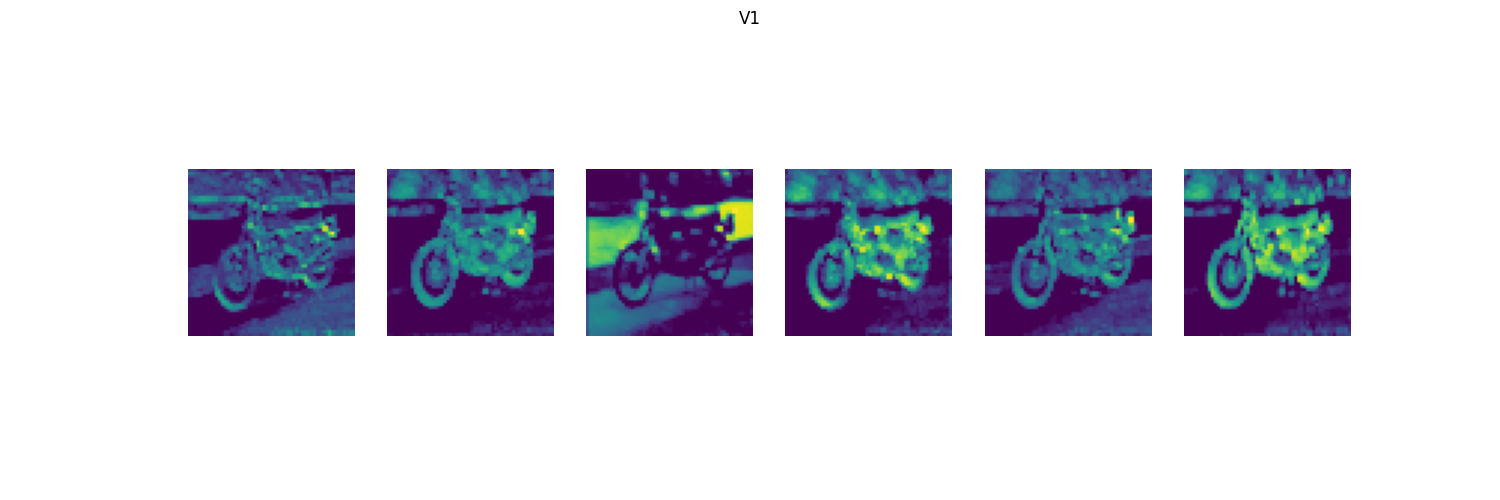
\includegraphics[width=0.8\linewidth]{V1_activations.png}
	\caption{CORnet-Z模型V1层激活图}
	\label{f.v1_act}
\end{figure}

随着网络加深,在V2图\ref{f.v2_act}与V4层图\ref{f.v4_act}中,激活图的结构逐渐从边缘线条过渡为较粗的区域块,表明模型开始提取更高级别的图像结构特征。

\begin{figure}[hbt]
	\centering
	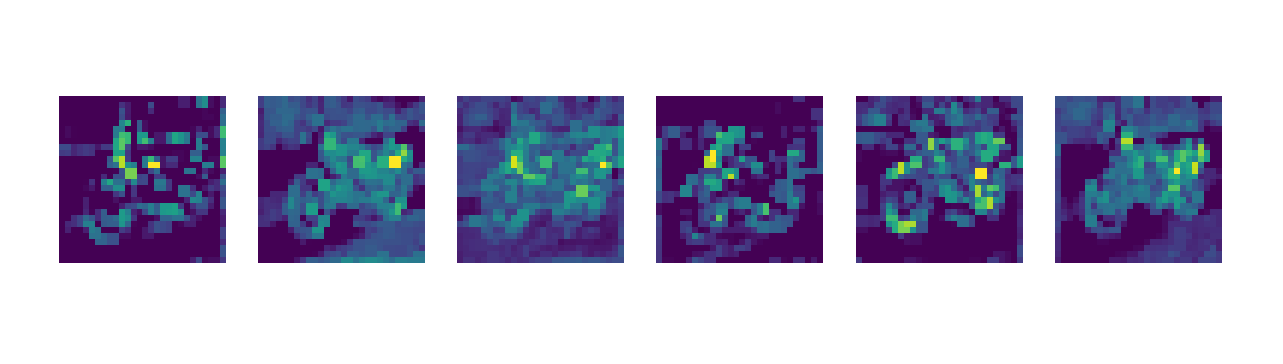
\includegraphics[width=0.8\linewidth]{V2_activations.png}
	\caption{CORnet-Z模型V2层激活图}
	\label{f.v2_act}
\end{figure}

\begin{figure}[hbt]
	\centering
	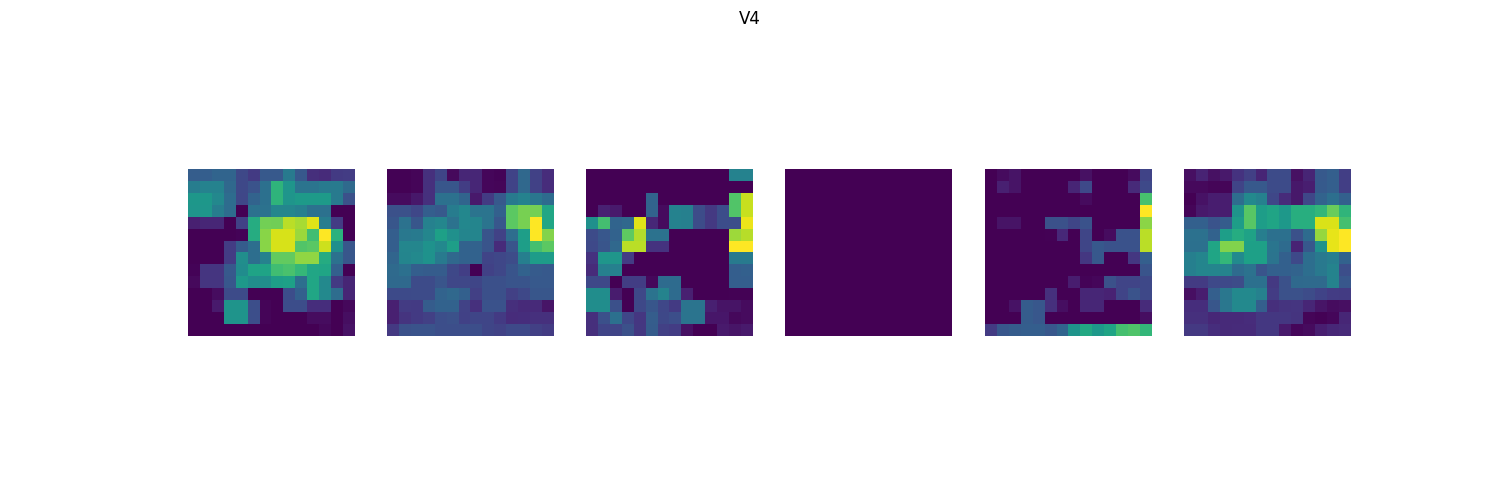
\includegraphics[width=0.8\linewidth]{V4_activations.png}
	\caption{CORnet-Z模型V4层激活图}
	\label{f.v4_act}
\end{figure}

\begin{figure}[hbt]
	\centering
	
\includegraphics[width=0.8\linewidth]{IT_activations.png}
	\caption{CORnet-Z模型IT层激活图}
	\label{f.it_act}
\end{figure}

在最高层IT图\ref{f.it_act}中,激活图整体变得更抽象,但依然可以观察到对目标核心区域的聚焦响应,表现出较强的语义抽象能力。不同通道间的激活存在差异,说明模型在高层仍保持了一定程度的特征多样性。

\subsection{引入SE机制后的激活变化}

在引入通道注意力机制后,模型的特征响应发生了明显变化。如图\ref{f.v1_se_act}所示,V1层的激活图较原始模型出现了显著压缩,部分通道的响应范围明显减小,整体响应区域更加集中。

\begin{figure}[hbt]
	\centering
	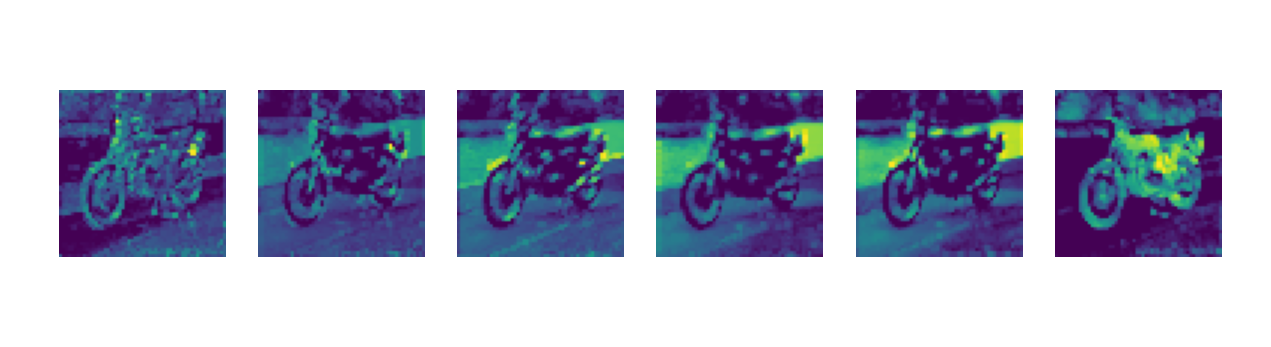
\includegraphics[width=0.8\linewidth]{V1_se_activations.png}
	\caption{CORnet-Z+SE模型V1层激活图}
	\label{f.v1_se_act}
\end{figure}

V2层图\ref{f.v2_se_act}表现出更零散的响应点分布,通道间响应差异增大,部分通道几乎无明显激活。

\begin{figure}[hbt]
	\centering
	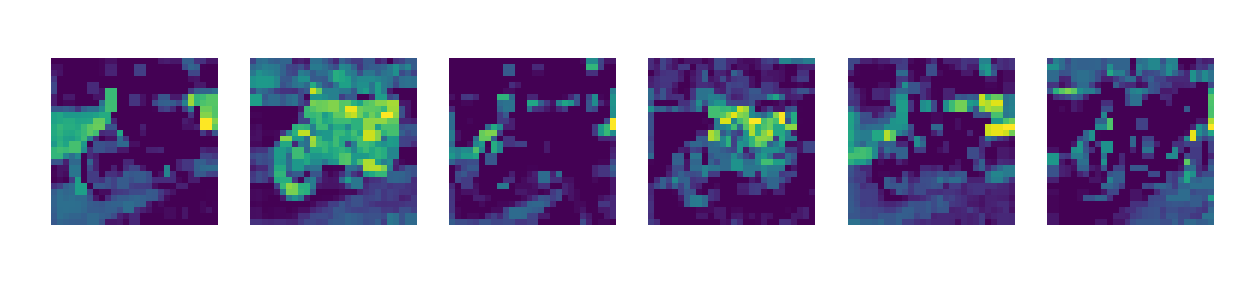
\includegraphics[width=0.8\linewidth]{V2_se_activations.png}
	\caption{CORnet-Z+SE模型V2层激活图}
	\label{f.v2_se_act}
\end{figure}

V4层图\ref{f.v4_se_act}进一步体现了这种稀疏化趋势,相较于CORnet-Z模型,SE版本在此层的高响应区域数量更少,许多通道的响应接近全黑。IT层激活图层图\ref{f.it_se_act}也呈现出类似特征,尽管部分通道对图像的核心区域产生了明显响应,但整体激活的多样性有所下降。

\begin{figure}[hbt]
	\centering
	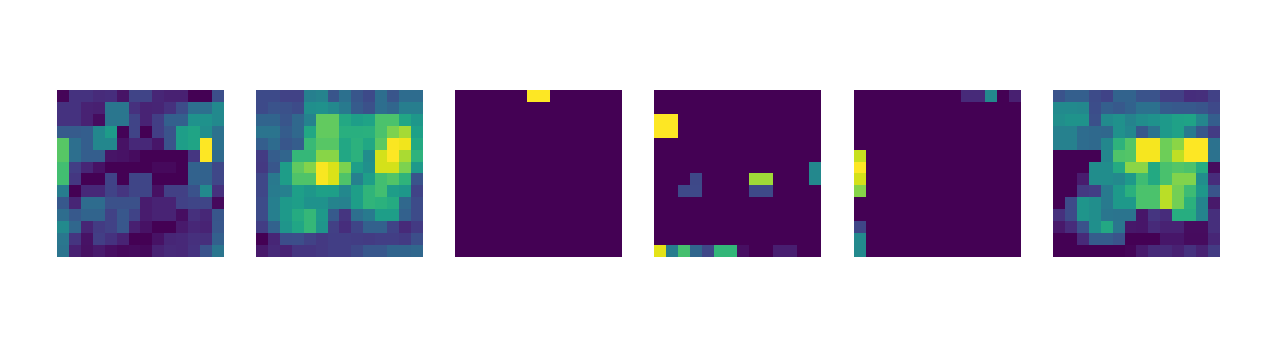
\includegraphics[width=0.8\linewidth]{V4_se_activations.png}
	\caption{CORnet-Z+SE模型V4层激活图}
	\label{f.v4_se_act}
\end{figure}

\begin{figure}[hbt]
	\centering
	
\includegraphics[width=0.8\linewidth]{IT_se_activations.png}
	\caption{CORnet-Z+SE模型IT层激活图}
	\label{f.it_se_act}
\end{figure}

这些变化说明,SE模块在网络中强化了部分重要通道的表达能力,同时抑制了其它通道的信息流。这种通道间的强弱选择虽然可能有助于提升分类性能,但也在一定程度上削弱了模型对图像整体结构的表达能力。

\subsection{局部目标关注能力分析}

综合观察可发现,SE模块增强了模型对图像中局部显著区域的响应能力。通过对比CORnet-Z与CORnet-Z+SE模型在V4层的激活图,可以发现注意力机制对局部目标特征的表征能力产生了显著影响。以第2个通道为例,原始模型在该通道中的激活图表现为零散分布,缺乏结构性。而在引入SE模块后,模型在相同通道上展现出更强的空间聚焦能力,激活区域更集中地覆盖于摩托车车身与轮胎等语义区域,抑制了背景部分的无效响应。

\begin{figure}[hbt]
	\centering
	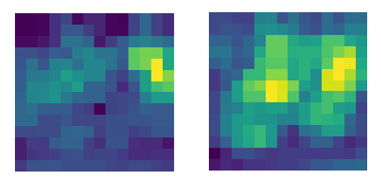
\includegraphics[width=0.6\linewidth]{V4层通道2对比图.png}
	\caption{V4层通道2对比图}
	\label{f.v4_2_act}
\end{figure}

然而,在类脑相似性方面,这种高度选择性的响应可能并不完全符合灵长类视觉皮层中多通道、分布式的响应模式。特别是在V4和IT层,SE模型在Brain-Score得分中的下降可能与激活图中体现出的稀疏性与响应单一性有关。

总体来看,原始CORnet-Z模型在各层的激活图表现出较好的层次演化特征,能够从底层边缘特征逐步整合到高层语义信息,而引入SE模块后虽然增强了判别性响应,但可能在整体特征覆盖和类脑表现方面有所取舍。
